\documentclass[a4paper, openany]{memoir}

\usepackage[utf8]{inputenc}
\usepackage[T1]{fontenc} 
\usepackage[english]{babel}
\usepackage{amsmath}
\usepackage{amssymb}

\usepackage{booktabs}
\usepackage{fancyhdr}
\usepackage{float}
\usepackage{indentfirst}
\usepackage{graphicx}
\usepackage[linewidth=1pt]{mdframed}
\usepackage{multicol}
\usepackage{fancyvrb}

\usepackage{longtable}

\pagestyle{fancy}
\fancyhf{}
\fancyhead[LE]{\leftmark}
\fancyhead[RO]{\rightmark}
\fancyhead[RE, LO]{PSD}
\fancyfoot[LE, RO]{\thepage}
\fancyfoot[RE, LO]{Pete Gautam}

\renewcommand{\headrulewidth}{1.5pt}

\setcounter{chapter}{15}
\chapterstyle{thatcher}

\begin{document}

\chapter{Software Refactoring}
It is easier to alter a software to respond as changes arise in the system's requirements and the environment if the source code has been carefully maintained. The characteristics of a well-maintained software include:
\begin{itemize}
    \item effective use of a version control system;
    \item an automated test suite;
    \item a clear architecture and design;
    \item a simple and consistent coding style, enforced through automation whenever possible; and
    \item appropriate use of comments and other documentation when absolutely necessary.
\end{itemize}

A key discipline for maintaining the structure of the software system is refactoring. It should be an ongoing process in a software development project alongside the introduction of new features. Refactoring is defined a change made to the internal structure of the software that makes it easier to understand and cheaper to modify while minimising the change in its observable behaviour. Refactoring often causes changes in the non-functional properties in the system, and might even cause changes in the functional behaviour or the specification.

\section{The refactoring process}
Refactoring can be thought of as a form of source code cleanup, with the addition of a well-defined process for performing the changes. The diagram below illustrates the process of refactoring.
\begin{figure}[H]
    \centering
    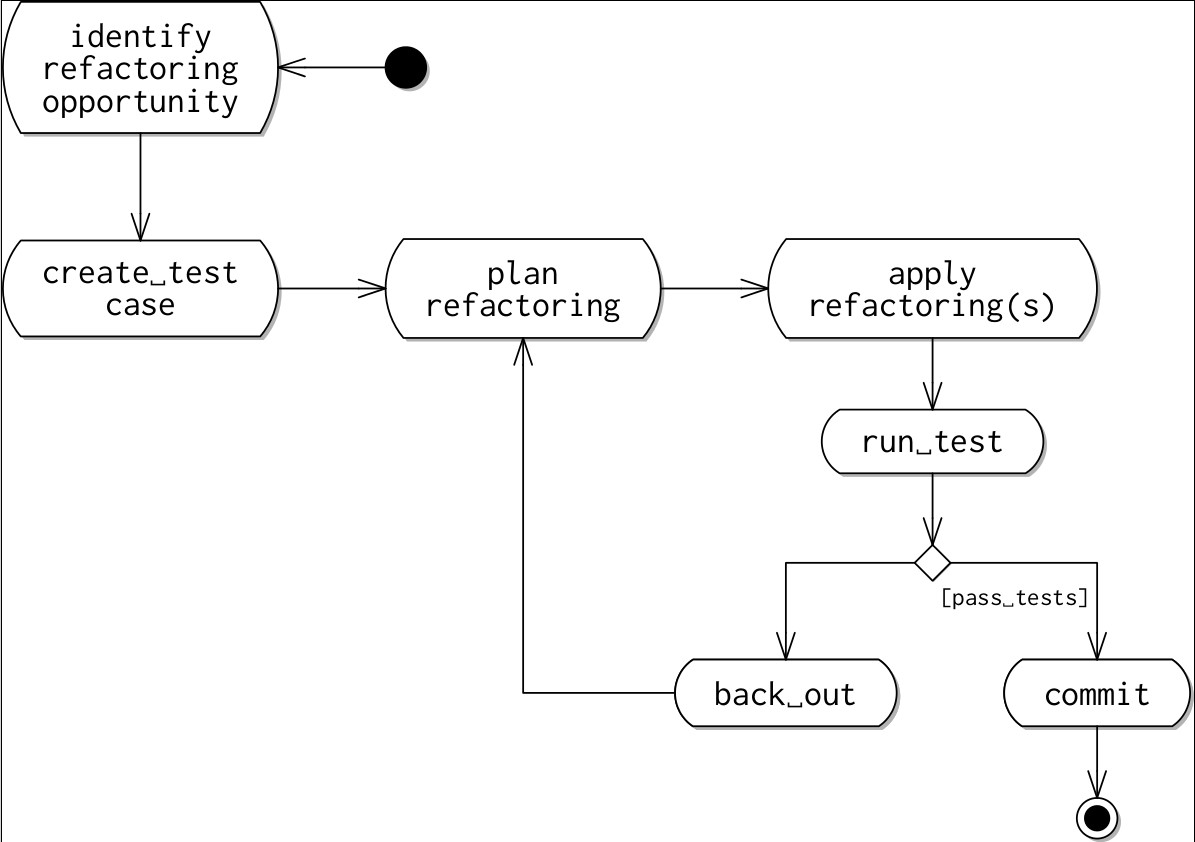
\includegraphics[scale=0.3]{src/16.1 refactoring process.png}
    \caption{The refactoring process}
\end{figure}
We start by identifying opportunities to refactor. These can be done by finding bad smells in the program. A bad smell is a pattern in the source code that indicates poor structure or inappropriate coupling between the modules.

Once an opportunity to refactor has been identified, it is important to create tests for affected classes. This can be done using an automated test framework such as PyUnit or Junit. Test cases are important because they will be used to show that the functional behaviour of the refactored code has not been changed as a result of applying any refactoring. 

Next, the refactoring is planned based on the guidance provided by the bad smells. Once the revised design has been established, they can be applied. This can often be done using automated refactoring tools that are provided as part of many IDEs, such as IntelliJ and PyCharm.

At this point, the tests developed previously should be run. If the code passes the tests, it is appropriate to commit the new design and the source code to the main project. If one or more of the tests fail, this indicates that the refactoring has altered the functional behaviour of the classes. In that case, we should back out of the changes, i.e. revert them. Additional planning and analysis can take place to understand what unexpected effect the refactoring has had. Once the revised design has been established, the revised refactorings can be applied. This process can be continued iteratively until a refactored system passes the pre-written tests.

\section{When to refactor}
Refactoring should be treated as a parallel, ongoing process that occurs alongside other software development activities. This means that we should be looking for opportunities to refactor when:
\begin{itemize}
    \item implementing a new functionality;
    \item correcting a defect;
    \item doing a code review; and
    \item trying to understand how a software artifact works.
\end{itemize}
While undertaking these tasks, we should also be observing for examples of poor software design in the source code. In particular, we should look out for bad smells. Bad smells are clues that the source code could be improved in some fashion.

\section{Bad smells}
We will now have a look at all the possible bad smells:
\begin{itemize}
    \item Cloning: This is when the source has been cloned rather than reused. This makes maintenance harder. In particular, if we find a bug in the original code, we have to fix all the clones as well.
    \item Complex structure: This is either a long method or a large class. 
    \begin{itemize}
        \item If a method is long, it gets harder to understand its behaviour because a lot of the details of the implementation are presented to the reader at once. In general, methods should only be a few lines long. 
        \item A large class might have too many responsibilities allocated to it. It is also possible for the large class to contain duplicate code.
    \end{itemize}
    \item Variables and parameters: There are many possible bad smells with variables and parameters.
    \begin{itemize}
        \item A long parameter list imposes a form of stamp coupling on the design of the method that they belong to. Each time the parameter list changes, every call of the method must also be changed. A long parameter list might also indicate that the method is used in different ways depending on how it is called.
        \item Feature envy indicates that a method is in the wrong class. This is because it obtains most of its data from another class. If either the data or the accessing method changes, the other one will also need to change.
        \item Data clumps occur when the same independently sourced data is used together in different locations within the system. It might be identifiable from duplicate parameter lists for methods, or from duplicate blocks of code for query method calls. Both of these are also examples of cloning.
        \item Primitive obsession indicates a preference for using primitive data types for representing more complex values with additional semantics. This is problematic because the semantics and other properties of data type are not made explicit when they are represented by primitive values; this has to be maintained independent of the data. For example, a date could be represented by 3 integers (day, month and year). But, this means that the relationship between the values (e.g. some constraint on the date) has to be maintained elsewhere in the system.
        \item Temporary field is where the fields are used as variables and method bodies, but aren't always needed. A field should only be used to record information about an object's state that must persist between method calls.
    \end{itemize}
    \item Making changes is about what has to be done when changes are made to the software.
    \begin{itemize}
        \item Divergent change indicates a class has too many responsibilities. This can be identified when a single class must be altered in different ways in order to respond to different changes in the system environment. This suggests that the class is fulfilling different sets of responsibilities.
        \item Shotgun surgery is the opposite of divergent change. This can be identified when a single change in the environment requires a number of different changes in several different classes. This makes maintenance time-consuming and it is easier to get wrong if we forget to make changes to one of the classes.
        \item Parallel inheritance hierarchies are identifiable by dependencies between 2 independent hierarchies such that a change in one hierarchy causes a change in the other. This increases coupling and maintenance costs. This can be thought of as a specialised form of shotgun surgery.
    \end{itemize}
    
    \item Control structures and polymorphism give rise to another family of bad smells.
    \begin{itemize}
        \item Switch statements indicate a reluctance to exploit object-oriented polymorphism and increases maintenance costs. Each time a new option is added to a switch, a flag and an additional line must be added.
        \item Sometimes, a subclass does not need all the methods provided by a superclass. This means that all the methods of the superclass are unnecessarily coupled to the sublcass. This is called refused bequest.
        \item Using alternative classes with different interfaces means that the benefits of object-oriented polymorphism cannot be exploited. Two or more classes must be manually selected for use in code rather than benefiting from a single consistent interface or operations.
    \end{itemize}
    
    \item Some bad smells are evidence that the software team was uncertain as to how their software design would eventually be used and what functionalities the different parts of the system would need to contain. This is design uncertainty.
    \begin{itemize}
        \item A lazy class is a class that has insufficient independent responsibilities. It can be unnecessarily expensive to maintain this class. 
        \item Although abstracting a concrete implementation detail is generally good, it can be tempting to move all the design decisions into the configuration for a software system. At its most extreme, this phenomenon is called the inner platform anti-pattern. The design is designed as a software platform that must be configured on top of an existing software platform. This called speculating generality, and involves the avoidance of design decisions to maintain generality for potential use in the future.
        \item Incomplete library class is not so much a smell, but can cause other smells. It occurs when we discover that a class from the library does not support all the operations needed by the client. Moreover, the library class cannot be altered because it is being used by many other projects.
    \end{itemize}
    
    \item Delegation is when one object attempts to delegate some of its responsibilities to another object.
    \begin{itemize}
        \item Message chains occur when a message from one object accesses data items through a series intermediary objects. The requesting object is therefore bound to all the objects in the chain.
        \item The middle man occurs when one objects as an information broker to another object, and does not provide any information itself. There may be a good reason to do this, e.g. if the broker is a proxy. If the object is merely passing objects on, it may be better for the communication to occur directly.
        \item Inappropriate intimacy (or object orgy anti-pattern) is the smell opposite to the middle man and message chains. Instead, all objects freely interact with the properties of other objects. This causes an orgy of couplings between them.
        \item Data class is a bad smell since classes should normally have behavioural responsibilities as well as data values in their state. If a class lacks any behaviour, this is often because the behaviour has been implemented somewhere else.
    \end{itemize}
\end{itemize}

Many of the bad smells and refactoring remedies are illustrative of the principles of good design. These principles embody the adage that a good design has low coupling and high cohesion. Refactoring is concerned with reducing the coupling and increasing the cohesion in a software application.

Another bad smell is excessive use of comments to explain the source code. Comments are indicative of a poor structure that could be improved through the application of refactorings. This process helps to create self-documenting code. Once the code has been refactored, its purpose and functionality should become much more evident. This reduces the need for supplementary documentation. Most of the documentation can be removed when the refactoring is complete.

\section{Types of refactoring}
To address bad smells, there is a wide range of refactoring plans that could be applied. 
\begin{itemize}
    \item Fixing methods: we can do this by either extracting a method from a very large method or by inlining a very small method back into the body of the method somewhere else. We can also replace a method with a method object.
    \item Moving functionality around a program: we can move a method or a field from one class to another. We can extract a class from a big class, or inline a class black into another class if it has sufficient responsibilities.
    \item Organising data: we can encapsulate fields, replace magic number with symbolic constant and replace data value with an object.
    \item Simplifying method calls: we can parametrise methods or remove a parameter if necessary. We can also make use of a parameter object.
    \item Simplifying conditions: we can decompose conditionals into subparts. We can consolidate duplicate conditional fragments into the same location or replace conditionals with polymorphism.
    \item Reorganising classes: we can pull a method or a field up or push it down the inheritance hierarchy. We can extract a superclass from a set of subclass or extract subclass from existing superclass, and collapse a hierarchy that is too large.
\end{itemize}

\section{Smells to refactor}
The following table summarises how to refactor each type of smell:
\begin{longtable}{p{0.3\linewidth} p{0.6\linewidth}}
    \hline
    Smell & Strategies \\
    \hline
    Duplicated code & extract method - (pull up method, form template method) or substitute algorithm \\
    \hline
    Long method & extract method - (introduce parameter object, replace temp with query) or replace method with method object - extract method \\
    \hline
    Large class & extract class, extract subclass \\
    \hline
    Long parameter list & replace parameter with method, preserve whole object \\
    \hline
    Divergent change & extract class \\
    \hline
    Shotgun surgery & move method, move field, inline class \\
    \hline
    Feature envy & move method, extract method \\
    \hline
    Data clumps & extract class - (introduce parameter object, preserve whole object) \\
    \hline
    Primitive obsession & replace data value with object, replace type code with class, extract class, introduce parameter object \\
    \hline
    Switch statements & replace type code with subclasses - replace conditional with polymorphism \\
    \hline
    Parallel inheritance hierarchies & move method, move field \\
    \hline
    Lazy class & collapse hierarchy, inline class \\
    \hline
    Speculative generality & collapse hierarchy, inline class, remove parameter, rename method \\
    \hline
    Temporary field & extract class, introduce null object \\
    \hline
    Message chains & hide delegate, extract method - move method \\
    \hline
    Middle man & remove middle man, inline method \\
    \hline
    Inappropriate intimacy & move method, move field, extract class, hide delegate, change bidirectional association to unidirectional, replace inheritance with delegation \\
    \hline
    Alternative classes with different interfaces & rename method, move method, extract superclass \\
    \hline
    Incomplete library class & introduce foreign method, introduce local extension \\
    \hline
    Data class & encapsulate field, extract method, move method, hide method \\
    \hline
    Refused bequest & push down method, push down field, replace inheritance with delegation \\
    \hline
\end{longtable}

\subsection{Refactoring the \texttt{Book} class}
We will now illustrate the refactoring strategy with an example. Assume that we have the following classes in Java.
\begin{figure}[H]
    \centering
    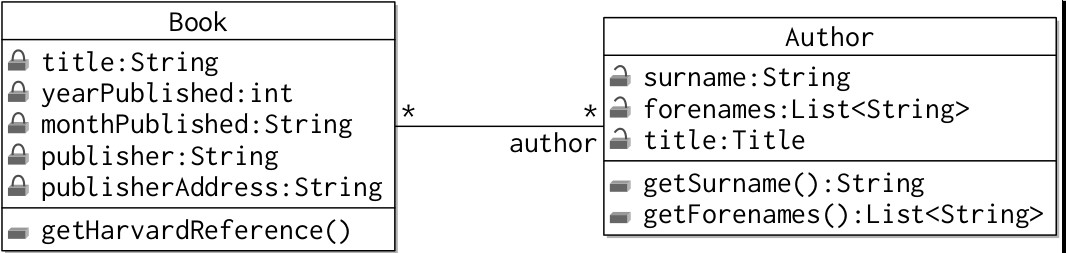
\includegraphics[scale=0.35]{src/16.2 book class before.png}
\end{figure}
\noindent The image illustrates the partial programming relationship between books (stored in the database) and their authors. The method \texttt{getHarvardReference} in the \texttt{Book} class is given below.
\begin{verbatim}
public String getHarvardReference(){
    String result = "";
    
    for (Author author: authors){
        String surname = author.getSurname();
        result+=surname + ", ";

        List<String> forenames = author.getForenames();
    
        for (String forename: forenames)
            result += forename.charAt(0)+".,";
    }
    result+=" ("+monthPublished+", "+yearPublished+") ";
    
    result+=title+". ";
    
    result+=publisherAddress+": "+publisher+".";
    return result;
}
\end{verbatim}
The purpose of this method is to format the details of the book in Harvard Referencing style. 

To start the refactoring process, we need to identify the bad smells. These are:
\begin{itemize}
    \item The method is too long. It contains a mixture of queries, processing and string composition.
    \item The method has primitive obsession- the attributes \texttt{yearPublished} and \texttt{monthPublished} are primitive attributes that should be within a \texttt{Date} object.
    \item There is data clumping. It is likely that the publisher's name and address will be used together, so this should be in its own method/class.
\end{itemize}

The next stage in the refactoring process is to construct the test cases to check whether the changes alter the correctness of the method. Then, we plan the refactorings based on the smells.
\begin{itemize}
    \item We apply `extract method' to the code for formatting the author's name and `move method' to the resulting method so it is in the \texttt{Author} class.
    \item We apply `replace data value with object' to the combined \texttt{yearPublished} and \texttt{monthPublished} attributes to deal with primitive obsession smell.
    \item We apply `extract class' to attributes concerning the book publisher.
    \item We apply `introduce parameter object' to the relevant String arguments in the constructor. This may introduce a lazy class, so it may be better to use `extract inline class'.
\end{itemize}
While performing the refactoring, several new lines of code are introduced to the method \texttt{getHarvardReference} to deal with extracting the year of publication from the published attribute. Also, the refactored code using extract method and move method can be applied to the code that now accesses and formats the publisher's details.

The refactoring also causes several changes to the test methods because the constructor has been changed. This is fine because the method under test has not been altered. The revised book class has the following class diagram:
\begin{figure}[H]
    \centering
    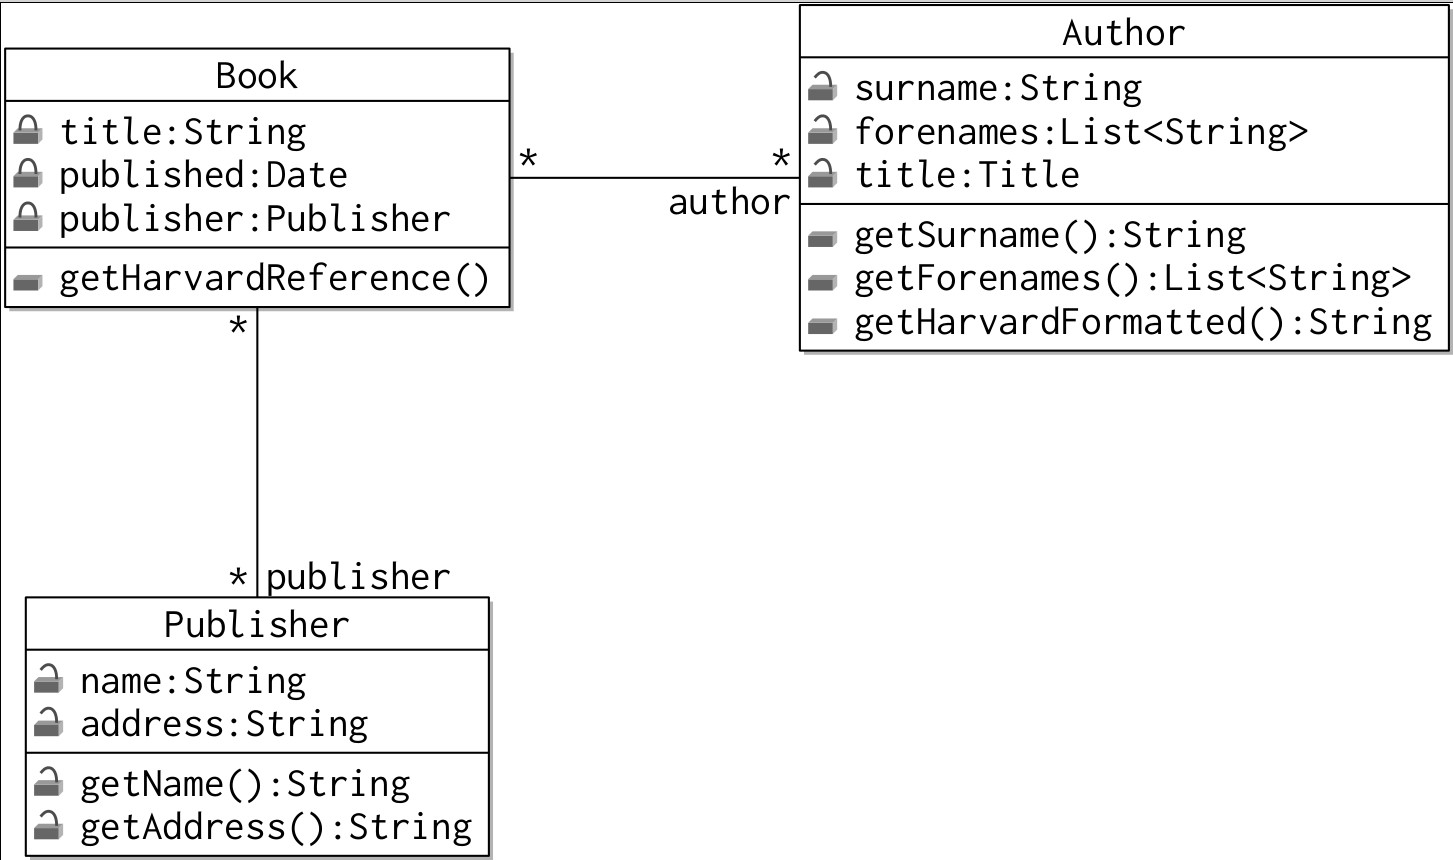
\includegraphics[scale=0.25]{src/16.3 book class refactored.png}
\end{figure}
\noindent We have moved the \texttt{getHarvardFormatted} method into \texttt{Author} class and created a new \texttt{Publisher} class. The code itself has been refactored to the following:
\begin{verbatim}
 public String getHarvardReference(){
    String authors = getHarvardFormattedAuthors();

    String publisherDetails =
        publisher.getHarvardFormatted();
    
    String datePublished = getDatePublished();
    
    String harvardFormat = "%s (%s) %s. %s";
    
    String result = 
        String.format(
            harvardFormat,authors,datePublished,
            title,publisherDetails);    
    
    return result;
}

private String getDatePublished() {     
    DateFormat dateFormat = new SimpleDateFormat("MMMM, yyyy");
    String result = dateFormat.format(published);
    return result;
}

private String getHarvardFormattedAuthors(){
    String result = "";
    for (Author author: authors)
        result += author.getHarvardFormatted();
    return result;
}
\end{verbatim}

Now, the method \texttt{getHardvardReference} delegates responsibility for formatting the author string to a separate method. Similarly, the publisher details come from the publisher object. The overall structure of the code is much simpler.

\section{Automated refactoring}
Many software tools, such as IDEs, have integrated tool support for automatic refactoring, e.g. Eclipse and IntelliJ have support for a wide variety of refactorings such as:
\begin{itemize}
    \item renaming artifacts;
    \item moving artifacts;
    \item extracting interface;
    \item extracting superclass;
    \item pulling a method/field up the inheritance hierarchy;
    \item pushing a method/field down the inheritance hierarchy;
    \item extracting class;
    \item changing the method signature;
    \item inlining a class;
    \item inlining a method;
    \item inlining a field;
    \item introducing a parameter object;
    \item introducing indirection;
    \item inferring generic-type arguments;
    \item generalising declared type; and
    \item encapsulating field.
\end{itemize}

\section{Limits of refactoring}
The refactoring process is a powerful mechanism for managing design and quality as the software and the application evolves. But, refactorings can themselves cause the software to evolve and consequently can alter the observable behaviour of the software system. 

Refactorings can cause observable changes to the software system in either the non-functional properties of the system or the API. Refactorings which cause changes to a non-functional property might decrease the system's overall memory footprint and the system's response time. This might be because the refactoring reduces the amount of cloning in a software system. Unfortunately, this may increase the number of method calls that must be made. This increases the execution time for a transaction.

These considerations are particularly important for mobile-embedded or real-time applications in which computing resources may be limited. However, a clear design is usually easier to tune. This way, over the long term, the required non-functional properties of the system are easier to achieve.

In addition to changing non-functional behaviour, some refactorings require an API to be altered. The API is a set of public operations and attributes of a module that can be accessed by other module systems at runtime. In object-oriented systems, every object has an API defined by the public members- the operation attributes of a class.

Changes to an API can happen in the following cases:
\begin{itemize}
    \item when a class member is moved;
    \item when a class member is renamed;
    \item when the visibility of a class memeber is changed;
    \item when the list of parameters to an operation is changed;
    \item when the return type of an operation is changed;
    \item when the exceptions that may be raised are changed;
\end{itemize}

This may not be a significant problem if the API is for a class that is only accessed within the software system. However, some APIs must be exposed to the users of the system. These are called published interfaces because they have been exposed and documented for use by the external clients of the software system.

Consequently, every user of the software system is coupled to the API specification. The version of the system used is a dependency to all its users. If the API specification is changed, then the part of the old API that has changed becomes deprecated. It must be discarded in a later release. We expect it to be retained at this moment so that the dependent systems have some time to update. Typically, the development team for a software system that has dependents issues a migration plan to explain how they can adapt the system to the new API.

In summary, refactoring is a key practice that should occur alongisde other software activities. Refactoring is a formalised form of code cleanup in which changes are made according to a well-specified process with respect to a predefined plan. Refactoring opportunities are detected through the occurrence of bad smells in code. Each bad smell can be remedied through the application of one or more refactorings. Applying a refactoring may lead to further opportunities to refactor.

\end{document}